\documentclass[10pt,letterpaper]{article}
\usepackage[utf8]{inputenc}
\usepackage[spanish,es-tabla]{babel}
\usepackage{geometry}
\geometry{margin=0.68in, top=0.85in, bottom=0.78in, headheight=36pt, headsep=14pt}
\usepackage{amsmath,amssymb}
\usepackage{xcolor}
\usepackage{graphicx}
\usepackage{tabularx}
\usepackage{booktabs}
\usepackage{colortbl}
\usepackage{array}
\usepackage{enumitem}
\usepackage{fancyhdr}
\usepackage{titlesec}
\usepackage{lastpage}
\usepackage{setspace}
\usepackage{listings}

% Tipografía institucional Icesi (Sans-Serif Helvetica)
\usepackage{helvet}
\renewcommand{\familydefault}{\sfdefault}

% Interlineado aumentado un 30% (setstretch 1.38) para mayor holgura y lectura óptima
\setstretch{1.38}

% Altura de celdas en tablas
\renewcommand{\arraystretch}{1.25}

% Paleta de Colores Oficial de los Programas Icesi
\definecolor{icesiBlue}{HTML}{5454E9}       % Azul vibrante institucional
\definecolor{icesiOrange}{HTML}{F0681A}     % Naranja acento
\definecolor{icesiGreen}{HTML}{4CB978}      % Verde acento
\definecolor{icesiPurple}{HTML}{865CF0}     % Púrpura acento
\definecolor{icesiDark}{HTML}{1A1A1A}       % Texto principal oscuro
\definecolor{icesiMuted}{HTML}{6B7280}      % Gris metadatos
\definecolor{icesiBorder}{HTML}{D1D5DB}     % Líneas y bordes
\definecolor{icesiRowLine}{HTML}{E5E7EB}    % Líneas de tabla
\definecolor{icesiLight}{HTML}{F9FAFB}      % Fondo suave
\definecolor{codeBackground}{HTML}{F3F4F6}  % Fondo código

% Configuración de Listings
\lstdefinestyle{bashstyle}{
    backgroundcolor=\color{codeBackground},
    commentstyle=\color{icesiMuted}\itshape,
    keywordstyle=\color{icesiBlue}\bfseries,
    basicstyle=\ttfamily\scriptsize,
    breaklines=true,
    frame=single,
    rulecolor=\color{icesiBorder},
    language=bash,
    showstringspaces=false
}

\lstdefinelanguage{Slice}{
  keywords={module, interface, class, struct, sequence, dictionary, exception, throws, idempotent, void, bool, byte, short, int, long, float, double, string, enum},
  sensitive=true,
  comment=[l]{//},
  morecomment=[s]{/*}{*/},
  morestring=[b]"
}

\lstdefinestyle{slicestyle}{
    backgroundcolor=\color{codeBackground},
    commentstyle=\color{icesiMuted}\itshape,
    keywordstyle=\color{icesiPurple}\bfseries,
    basicstyle=\ttfamily\scriptsize,
    breaklines=true,
    frame=single,
    rulecolor=\color{icesiBorder},
    language=Slice,
    showstringspaces=false
}

% =========================================================================
% ENCABEZADO Y PIE DE PÁGINA ESTILO PROGRAMA DE CURSO ICESI
% =========================================================================
\pagestyle{fancy}
\fancyhf{}
\fancyhead[L]{%
  \begin{minipage}[c]{2.8cm}
    
\includegraphics[height=0.82cm]{logo-icesi.png}
  \end{minipage}%
  \begin{minipage}[c]{12.2cm}
    \footnotesize\textbf{\color{icesiDark}UNIVERSIDAD ICESI --- FACULTAD DE INGENIERÍA, DISEÑO Y CIENCIAS APLICADAS}\\[-0.5mm]
    \scriptsize\color{icesiMuted}Departamento de Computación y Sistemas Inteligentes $\vert$ Computación en Internet I (09810 - TIC)
  \end{minipage}%
}
\fancyhead[R]{}

\fancyfoot[L]{%
  \begin{minipage}[c]{0.52\textwidth}
    \tiny\color{icesiMuted}\textbf{Proyecto Final:} Sistema Distribuido de Reserva de Boletas (ZeroC Ice \& Vanilla JS)
  \end{minipage}%
}
\fancyfoot[R]{%
  \tiny\bfseries\color{icesiMuted}Página \thepage\ de \pageref{LastPage}
}
\renewcommand{\headrulewidth}{0pt}
\renewcommand{\footrulewidth}{0.4pt}

\newcommand{\sectionBadge}[1]{%
  \refstepcounter{section}%
  \vspace{0.24cm}%
  \noindent%
  \colorbox{icesiBlue}{\color{white}\rule[-0.08cm]{0pt}{0.42cm}\hspace{0.16cm}\textbf{\normalsize \thesection}\hspace{0.16cm}}%
  \hspace{0.18cm}%
  {\fontsize{9.5}{12}\selectfont\textbf{\color{icesiDark}#1}}\\[-0.10cm]%
  \noindent{\color{icesiDark}\rule{\textwidth}{0.8pt}}\vspace{0.10cm}%
}

\titleformat{\subsection}
  {\color{icesiBlue}\normalfont\normalsize\bfseries}
  {\thesubsection}{0.4em}{}
\titlespacing*{\subsection}{0pt}{0.6ex plus 0.2ex minus .1ex}{0.2ex plus .1ex}

\begin{document}

% Barra decorativa superior multicolor institucional
\noindent
\begin{minipage}{\textwidth}
  \vspace{-10pt}
  \definecolor{barBlue}{HTML}{5454E9}
  \definecolor{barOrange}{HTML}{F0681A}
  \definecolor{barGreen}{HTML}{4CB978}
  \definecolor{barPurple}{HTML}{865CF0}
  \noindent\color{barBlue}\rule{0.25\textwidth}{3.5pt}%
  \color{barOrange}\rule{0.25\textwidth}{3.5pt}%
  \color{barGreen}\rule{0.25\textwidth}{3.5pt}%
  \color{barPurple}\rule{0.25\textwidth}{3.5pt}%
  \vspace{8pt}
\end{minipage}

% Título Principal
\begin{center}
  {\Large\bfseries\color{icesiDark}PROYECTO FINAL INTEGRADOR: SISTEMA DISTRIBUIDO DE}\\[1.5mm]
  {\Large\bfseries\color{icesiBlue}RESERVA DE BOLETERÍA CON ZEROC ICE \& VANILLA JS (WEBPACK)}\\[3mm]
  {\small\color{icesiMuted}\textbf{Arquitectura Híbrida RPC (TCP/WebSocket) $\vert$ Concurrencia $\vert$ Componentes Modulares}}
\end{center}

\vspace{2pt}

% Tabla de Metadatos del Proyecto
\noindent
\begin{tabularx}{\textwidth}{@{}|lX|lX|@{}}
\hline
\rowcolor{icesiLight}
\textbf{\scriptsize Código Asignatura:} & \scriptsize 09810 - TIC & \textbf{\scriptsize Período Académico:} & \scriptsize 2026-2 \\
\hline
\textbf{\scriptsize Grupo / NRC:} & \scriptsize NRC 12378  \\
\hline
\rowcolor{icesiLight}
\textbf{\scriptsize Ponderación:} & \scriptsize 20.0\% (Proyecto Final del Curso) & \textbf{\scriptsize Política IAG:} & \scriptsize Nivel 3: Colaboración Asistida \\
\hline
\textbf{\scriptsize Integrante:} & \scriptsize & \textbf{\scriptsize Código 1:} & \scriptsize \\
\hline
\end{tabularx}

\vspace{10pt}

% =========================================================================
% SECCIÓN 1: CONTEXTO DEL PROBLEMA Y ARQUITECTURA DISTRIBUIDA
% =========================================================================
\sectionBadge{Contexto del Problema y Arquitectura del Sistema}

Las plataformas de comercio electrónico de alta demanda, tales como las taquillas virtuales para conciertos masivos y eventos deportivos, representan uno de los mayores desafíos en la ingeniería de sistemas distribuidos. En estos entornos, decenas de miles de usuarios acceden simultáneamente al abrirse la boletería, compitiendo por un número finito de asientos con la expectativa de una experiencia interactiva en tiempo real y garantías absolutas de consistencia que eviten el \textit{overbooking} (sobreventa).

Para este proyecto integrador, los estudiantes construirán un Sistema Distribuido de Reserva de Boletas denominado \textbf{Icesi Live Arena}, articulando dos grandes paradigmas:
\begin{enumerate}[leftmargin=*]
  \item \textbf{Backend de Alta Disponibilidad en Java (ZeroC Ice):} Expone un servicio RPC (\textit{Remote Procedure Call}) multi-protocolo que atiende solicitudes concurrentes tanto en canal binario TCP (para clientes nativos) como en canal WebSocket (para clientes web).
  \item \textbf{Frontend Modular en JavaScript o TypeScript Vainilla con Webpack:} Una Single Page Application (SPA) construida enteramente en JavaScript o TypeScript moderno (ES6+), estructurada mediante Componentes Reutilizables y Módulos, sin frameworks (sin React, Vue ni Angular). Dicha aplicación se empaquetará profesionalmente mediante Webpack.
\end{enumerate}

\begin{center}
\small
\begin{tabularx}{0.96\textwidth}{@{}|l|l|X|@{}}
\hline
\rowcolor{icesiLight}
\textbf{Capa de Software} & \textbf{Tecnología y Protocolo} & \textbf{Responsabilidad en el Sistema} \\
\hline
\textbf{Frontend Web} & Vanilla JS (ES Modules) + Webpack & Plano interactivo de sillas, carrito reactivo, temporizadores y modal de checkout. \\
\hline
\textbf{Canal WebSocket} & \texttt{ws://localhost:10002} (ZeroC Ice) & Conexión RPC bidireccional desde el navegador hacia el servidor. \\
\hline
\textbf{Canal TCP} & \texttt{default -p 10000} (ZeroC Ice) & Canal para clientes nativos y batería de pruebas automatizadas. \\
\hline
\textbf{Servidor de Lógica} & Java 17 + ZeroC Ice 3.7 & Gestión del aforo (90 sillas), bloqueo temporal y confirmación de compra. \\
\hline
\end{tabularx}
\end{center}

\vspace{4pt}

% =========================================================================
% SECCIÓN 2: ESPECIFICACIÓN DEL BACKEND Y SERVICIOS RPC
% =========================================================================
\sectionBadge{Especificación del Backend y Servicios RPC}

\subsection{Servicios Implementados en el Backend (Contrato Slice)}

El servidor expone la interfaz remota \texttt{BookingService} definida en el archivo \texttt{BookingService.ice}. Esta interfaz encapsula las operaciones fundamentales para la consulta del recinto, reserva temporal y confirmación transaccional:

\begin{center}
\scriptsize
\begin{tabularx}{\textwidth}{@{}|l|p{3.2cm}|l|X|@{}}
\hline
\rowcolor{icesiLight}
\textbf{Operación RPC} & \textbf{Parámetros de Entrada} & \textbf{Retorno} & \textbf{Descripción y Excepciones} \\
\hline
\texttt{getEventInfo()} & \textit{Ninguno} & \texttt{EventInfo} & Retorna la metadata del concierto (nombre, fecha, aforo total de 90 sillas, precios por zona y contadores de sillas disponibles, bloqueadas y vendidas). \\
\hline
\texttt{getAllSeats()} & \textit{Ninguno} & \texttt{SeatList} (\texttt{Seat[]}) & Retorna la lista completa de las 90 sillas con su identificación, zona, fila, número, precio, estado y cliente retenedor. \\
\hline
\texttt{getSeatsByZone(zone)} & \texttt{SeatZone zone} & \texttt{SeatList} (\texttt{Seat[]}) & Retorna las sillas filtradas por zona: \texttt{ZONEVIP}, \texttt{ZONEPLATEA} o \texttt{ZONEGENERAL}. \\
\hline
\texttt{getSeat(seatId)} & \texttt{string seatId} & \texttt{Seat} & Consulta el detalle de una silla específica por código (ej. \texttt{"A-1"}). Lanza \texttt{SeatNotFoundException} si no existe. \\
\hline
\texttt{lockSeat(seatId, clientId)} & \texttt{string seatId}\newline\texttt{string clientId} & \texttt{LockResult} & Bloquea temporalmente una silla disponible por 90 segundos para el cliente indicado. Si el mismo cliente reintenta, renueva el tiempo. Lanza \texttt{SeatNotFoundException} o \texttt{SeatNotAvailableException}. \\
\hline
\texttt{releaseSeat(seatId, clientId)} & \texttt{string seatId}\newline\texttt{string clientId} & \texttt{bool} & Libera voluntariamente el bloqueo temporal de una silla antes de que expire su tiempo. Retorna \texttt{true} si la operación fue exitosa. Lanza \texttt{SeatNotFoundException}. \\
\hline
\texttt{confirmBooking(seatIds, clientId, name, email)} & \texttt{StringSeq seatIds}\newline\texttt{string clientId}\newline\texttt{string customerName}\newline\texttt{string customerEmail} & \texttt{BookingResult} & Confirma la compra definitiva de los asientos bloqueados, cambia su estado a \texttt{BOOKED} y genera un código de reserva (\texttt{RES-XXXXXX}). Lanza \texttt{InvalidBookingException} o \texttt{BookingException}. \\
\hline
\texttt{getMyLockedSeats(clientId)} & \texttt{string clientId} & \texttt{SeatList} & Retorna las sillas actualmente retenidas por el cliente cuyo temporizador se encuentre activo. \\
\hline
\texttt{getMyBookings(clientId)} & \texttt{string clientId} & \texttt{BookingList} & Retorna el historial de compras confirmadas realizadas por el cliente con sus respectivos códigos y totales. \\
\hline
\texttt{resetSeats()} & \textit{Ninguno} & \texttt{void} & Restablece el inventario a estado inicial (todas disponibles). Utilidad para pruebas de laboratorio. \\
\hline
\end{tabularx}
\end{center}

\subsection{Ciclo de Vida de los Asientos y Política de Bloqueo}
Cada una de las 90 sillas del auditorio (20 VIP, 30 Platea y 40 General) transita por tres estados:
\begin{itemize}[leftmargin=*]
  \item \textbf{AVAILABLE (Disponible):} La silla está libre para cualquier cliente.
  \item \textbf{LOCKED (Bloqueo Temporal de 90 Segundos):} Al seleccionarse, el cliente adquiere un derecho de compra exclusivo temporal. Si el tiempo expira sin confirmarse el pago, la silla se libera automáticamente para otros usuarios.
  \item \textbf{BOOKED (Venta Definitiva):} Una vez confirmado el pago, la silla queda asignada de forma irreversible con su respectivo código de reserva alfanumérico (\texttt{RES-XXXXXX}).
\end{itemize}

\vspace{4pt}

% ================================5.2 Fase 2: Estructura del Frontend y Bundling con Webpack (Semana 2)=========================================
% SECCIÓN 3: REQUERIMIENTOS DEL SISTEMA (FUNCIONALES Y NO FUNCIONALES)
% =========================================================================
\sectionBadge{Requerimientos del Sistema (Funcionales y No Funcionales)}

\subsection{Requerimientos Funcionales (RF)}
\begin{enumerate}[label=\textbf{RF-\arabic*:}, leftmargin=*]
  \item \textbf{Visualización de Aforo y Precios en Tiempo Real:} El sistema debe consultar y presentar la información del evento, precios por zona y el estado en tiempo real de las 90 sillas del recinto (Disponibles, Bloqueadas y Vendidas).
  \item \textbf{Selección y Bloqueo Temporal Exclusivo:} Al seleccionar un asiento disponible, el sistema debe solicitar su retención temporal exclusiva por 90 segundos al backend RPC. Dos usuarios no pueden bloquear la misma silla simultáneamente.
  \item \textbf{Temporizador Reactivo y Desbloqueo Automático:} La interfaz debe presentar una cuenta regresiva clara del tiempo restante de reserva. Al expirar los 90 segundos sin confirmación de compra, el asiento debe liberarse automáticamente en el servidor y quedar disponible para otros clientes.
  \item \textbf{Gestión de Carrito y Liberación Manual:} El usuario debe poder revisar las sillas en su carrito y removerlas voluntariamente antes de la expiración, liberándolas de inmediato en el backend mediante \texttt{releaseSeat}.
  \item \textbf{Checkout y Confirmación de Compra:} El usuario debe ingresar sus datos de contacto (nombre y correo electrónico válido) para confirmar la compra de sus sillas retenidas. El sistema debe validar que los bloqueos continúen vigentes, cambiar el estado a \texttt{BOOKED} y generar un código de reserva alfanumérico único (\texttt{RES-XXXXXX}).
  \item \textbf{Consulta de Reservas del Cliente:} El cliente debe poder consultar las compras confirmadas asociadas a su identificador de sesión.
  \item \textbf{Manejo Resiliente de Excepciones Remotas:} La interfaz debe capturar y notificar adecuadamente errores RPC del backend (sillas no disponibles, bloqueos expirados, desconexión del servidor) sin degradar la aplicación ni perder el estado local consistente.
\end{enumerate}

\subsection{Requerimientos No Funcionales y Restricciones Técnicas (RNF)}
\begin{enumerate}[label=\textbf{RNF-\arabic*:}, leftmargin=*]
  \item \textbf{Consistencia e Integridad Concurrente (Thread-Safety):} El backend debe garantizar exclusión mutua estricta en las operaciones críticas de inventario. Bajo ninguna condición de estrés concurrente se debe permitir el doble bloqueo o sobreventa de una misma silla.
  \item \textbf{Arquitectura Frontend en Vanilla JS (ES6+ / TypeScript):} El frontend debe implementarse exclusivamente en JavaScript moderno (ES6+) o TypeScript sin frameworks (prohibido el uso de React, Angular, Vue o similares). El código debe organizarse en componentes desacoplados con responsabilidades únicas.
  \item \textbf{Tooling y Empaquetado Profesional con Webpack:} El ciclo de vida del frontend debe administrarse con \texttt{npm} y empaquetarse con Webpack, proveyendo scripts \texttt{npm start} (desarrollo en puerto 3000) y \texttt{npm run build} (bundle optimizado para producción en \texttt{dist/}).
  \item \textbf{Interoperabilidad RPC Multi-Protocolo:} El cliente web debe comunicarse con el backend exclusivamente mediante el canal WebSocket (\texttt{ws://localhost:10002}) empleando la librería oficial de ZeroC Ice para JavaScript, mientras que el canal TCP nativo (\texttt{10000}) se reserva para pruebas automatizadas.
\end{enumerate}

\vspace{4pt}

% =========================================================================
% SECCIÓN 4: ESPECIFICACIÓN DEL FRONTEND EN JAVASCRIPT VAINILLA CON WEBPACK
% =========================================================================
\sectionBadge{Especificación del Frontend en JavaScript Vainilla con Webpack}

\subsection{Tooling y Empaquetado con Webpack}
El frontend debe gestionarse mediante \texttt{npm} e incluir los siguientes elementos:
\begin{enumerate}[leftmargin=*]
  \item \textbf{Gestor de paquetes:} Archivo \texttt{package.json} estructurado con dependencias de desarrollo (\texttt{webpack}, \texttt{webpack-cli}, \texttt{webpack-\allowbreak dev-\allowbreak server}, loaders de CSS y HTML) y dependencias de ejecución (\texttt{ice}).
  \item \textbf{Configuración Webpack (\texttt{webpack.config.js}):} Configuración que soporte ES Modules, bundle unificado, inyección automática de HTML y servidor de desarrollo en puerto \texttt{3000}.
  \item \textbf{Scripts de npm:} Comandos \texttt{npm start} (entorno de desarrollo) y \texttt{npm run build} (generación de la distribución de producción en \texttt{dist/}).
\end{enumerate}

\subsection{Guía de Interfaz (Wireframe de Referencia)}
La Figura~\ref{fig:mockup_componentes} presenta un \textit{wireframe} conceptual de referencia para el flujo de usuario en la aplicación. Este esquema ilustra las interacciones esenciales contempladas en los requerimientos del sistema: la visualización general del evento y aforo en tiempo real, el plano interactivo de selección de asientos con sus diferentes estados de ocupación, el panel lateral con la cuenta regresiva del bloqueo temporal y el formulario modal para la confirmación de la compra con su respectivo comprobante.

\vspace{4pt}
\noindent\textbf{Libertad de diseño y propuesta de componentes:} El prototipo suministrado tiene fines exclusivamente orientativos. Los estudiantes cuentan con total libertad para diseñar y proponer disposiciones visuales, jerarquías de elementos o estilos alternativos, siempre y cuando satisfagan a cabalidad los requerimientos funcionales y no funcionales definidos en la Sección~3. Es responsabilidad del equipo de estudiantes realizar el análisis de interfaz correspondiente y definir autónomamente la descomposición en componentes modulares y desacoplados dentro de su implementación en JavaScript o TypeScript vainilla.

\begin{figure}[htbp]
  \centering
  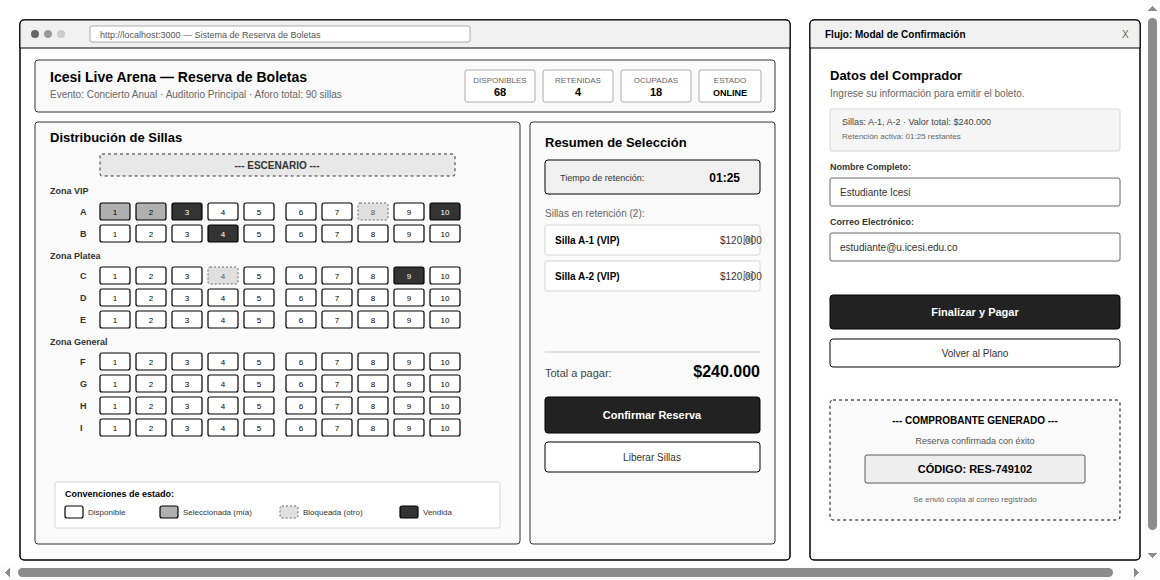
\includegraphics[width=\textwidth]{mockup_componentes.png}
  \caption{Wireframe de referencia para la interfaz de reserva de boletas y flujo de confirmación.}
  \label{fig:mockup_componentes}
\end{figure}

\vspace{2pt}

% =========================================================================
% SECCIÓN 5: PROCEDIMIENTO EXPERIMENTAL Y TAREAS POR FASES
% =========================================================================
\sectionBadge{Procedimiento de Desarrollo y Tareas por Fases}

El proyecto está diseñado para desarrollarse de manera progresiva:

\subsection{Fase 1: Estructura del Frontend y Bundling con Webpack (Sesión 1)}
\begin{enumerate}[leftmargin=*]
  \item Crear la carpeta \texttt{client-js/} e inicializar el proyecto con \texttt{npm init -y}.
  \item Instalar Webpack y los loaders necesarios (\texttt{html-webpack-plugin}, \texttt{style-loader}, \texttt{css-loader}, \texttt{ice}).
  \item Configurar \texttt{webpack.config.js} y validar la ejecución del entorno de desarrollo con \texttt{npm start} en el puerto \texttt{3000}.
  \item Diseñar y desarrollar la estructura modular de la interfaz en JavaScript o TypeScript con estilos desacoplados, implementando los módulos y componentes requeridos para el plano de asientos, temporizador reactivo y confirmación de compra.
\end{enumerate}

\subsection{Fase 2: Integración RPC con ZeroC Ice vía WebSocket y Validación E2E (Sesión 2)}
\begin{enumerate}[leftmargin=*]
  \item Configurar el cliente Webpack para inicializar el Communicator de ZeroC Ice y conectarse al endpoint WebSocket en \texttt{ws://localhost:10002}.
  \item Vincular los eventos de clic del plano con las llamadas remotas \texttt{lockSeat} y \texttt{releaseSeat}.
  \item Implementar la cuenta regresiva reactiva de 90 segundos con liberación automática ante expiración.
  \item Conectar el flujo de checkout con \texttt{confirmBooking} y desplegar el comprobante con el código de reserva.
  \item Realizar pruebas de usuario concurrentes abriendo múltiples ventanas de navegador en paralelo para comprobar la consistencia visual y remota del inventario.
\end{enumerate}

\vspace{6pt}

% =========================================================================
% SECCIÓN 6: CRITERIOS DE EVALUACIÓN Y SUSTENTACIÓN ORAL
% =========================================================================
\sectionBadge{Criterios de Evaluación y Sustentación Oral}

\subsection{Criterios de Evaluación Técnica del Proyecto (Nota Base)}
La solución técnica entregada se evaluará con base en los siguientes criterios sobre una escala base de \textbf{0.0 a 5.0 puntos}:

\vspace{2pt}
\begin{center}
\renewcommand{\arraystretch}{1.25}
\begin{tabularx}{0.75\textwidth}{|X|c|}
\hline
\rowcolor{icesiLight}
\textbf{Criterio de Evaluación} & \textbf{Porcentaje} \\
\hline
Tooling y Webpack & 20\% \\
\hline
Arquitectura Frontend Vanilla JS & 20\% \\
\hline
Integración RPC ZeroC Ice & 20\% \\
\hline
Concurrencia y Thread-Safety & 20\% \\
\hline
UX, Temporizador y Compra & 20\% \\
\hline
Despliegue en una VM de la sala & 10\% adicional \\
\hline
\rowcolor{icesiLight}
\textbf{Total} & \textbf{100\%} \\
\hline
\end{tabularx}
\end{center}

El despliegue aplica para quienes hicieron el despliegue el 8 de noviembre o lo realicen y sustenten para esta entrega.

\vspace{6pt}
\subsection{Sustentación Oral Individual (Factor Multiplicativo)}
La sustentación oral es de carácter estrictamente individual y se aplica como un \textbf{factor multiplicativo} ($F_s \in [0.0,\, 1.0]$) sobre la nota base obtenida por el proyecto en la evaluación técnica:

\begin{equation*}
\text{Calificación Definitiva Individual} = \text{Nota Base del Proyecto} \times F_s
\end{equation*}

\noindent
El factor de sustentación ($F_s$) evalúa la solvencia conceptual, la autoría del código y la argumentación de las decisiones de diseño mediante preguntas técnicas y posibles modificaciones en vivo formuladas por el docente:

\begin{itemize}[leftmargin=*, itemsep=2pt]
  \item \textbf{$F_s = 1.0$ (100\%):} Dominio técnico sobresaliente de la arquitectura global (backend ZeroC Ice, empaquetado con Webpack, sincronización de hilos y manipulación del DOM). Justifica con claridad todas las decisiones de diseño y responde con solidez a preguntas teóricas o modificaciones en vivo.
  \item \textbf{$F_s = 0.7 - 0.9$ (70\% -- 90\%):} Buen dominio general del funcionamiento del sistema, aunque con dudas leves o imprecisiones al explicar detalles técnicos puntuales de la implementación.
  \item \textbf{$F_s = 0.4 - 0.6$ (40\% -- 60\%):} Dominio técnico limitado o parcial. Dificultad para justificar segmentos clave del código entregado o evidencia de dependencia excesiva en otros integrantes del equipo.
  \item \textbf{$F_s = 0.0 - 0.3$ (0\% -- 30\%):} Desconocimiento sustancial del código fuente, incapacidad de explicar los flujos básicos de la aplicación o inasistencia no justificada a la sustentación oral.
\end{itemize}

\vspace{6pt}

% =========================================================================
% SECCIÓN 7: INSTRUCCIONES DE ENTREGA
% =========================================================================
\sectionBadge{Instrucciones y Políticas de Entrega}

\begin{enumerate}[leftmargin=*]
  \item \textbf{Repositorio de Código:} La entrega se realiza a través del repositorio Git enlazado en la organización del curso. La raíz del proyecto debe incluir:
    \begin{itemize}
      \item \texttt{codigo\_base/}: Con el servidor Java y la vulnerabilidad de concurrencia debidamente corregida y probada.
      \item \texttt{client-js/}: Con el proyecto frontend completo, configuración de Webpack, componentes y estilos.
    \end{itemize}
  \item \textbf{Historial de Commits:} Se exige un historial continuo con mensajes descriptivos bajo el estándar \textit{Conventional Commits} (\texttt{feat}, \texttt{fix}, \texttt{refactor}).
  \item \textbf{Video Demostrativo (Screencast):} Enlace a un video público o institucional de máximo 6 minutos demostrando:
    \begin{itemize}
      \item La ejecución del servidor Java y la prueba de estrés de concurrencia corregida.
      \item La compilación y ejecución de la aplicación web con \texttt{npm start} mediante Webpack.
      \item El flujo completo de navegación, bloqueo de sillas, cuenta regresiva del temporizador y emisión de la reserva.
    \end{itemize}
  \item \textbf{Sustentación Oral:} Cada estudiante presentará y defenderá su proyecto de forma presencial o sincrónica en el laboratorio en la fecha estipulada, donde se evaluará individualmente el factor multiplicativo $F_s$.
\end{enumerate}

\end{document}
